\section{Results}\label{sec:results}

The results follow the three problems of Section~\ref{sec:intro}: a comparison with common practice (Section~\ref{sec:res:common}), repairing reports (Sections~\ref{sec:res:readout} to \ref{sec:res:view}), detecting errors (Section~\ref{sec:res:persist}), and judging which report or configuration is more accurate (Sections~\ref{sec:res:select} and \ref{sec:res:transfer}). Each table caption states the operation, the comparator, the loss and any label use.

\subsection{Against common practice}\label{sec:res:common}

\begin{table*}[tp]\centering\footnotesize\setlength{\tabcolsep}{3pt}
\caption{Against common practice, from stored calls only. Columns give one call, the usual remedies (self-consistency: median of three stated counts, or a vote of three clicks; uncertainty-gated zoom: zoom only when two clicks disagree; majority vote and equal-weight box fusion over three calls), and our default. Relative changes are against one call, lower is better. \textbf{Bold}: the paired 95\% interval excludes 0 in the favourable direction; \underline{underlined}: it excludes 0 in the unfavourable direction. Our count readout costs about as much as one call and our click protocol less than a three-call vote. For Gemini 3.8, ``ours'' is the list-first protocol at its lowest setting; the method runs Gemini 3.8 at its default setting, which at the same 16k cap gives a readout error of 24.52 (Section~\ref{sec:res:degen}). For F1 our default is one call; over the 15 over-reporting cells, majority vote and box fusion change F1 by a median of $-0.3\%$ and $+0.2\%$. Per-cell set errors are in the released analysis outputs.}\label{tab:common}
\begin{tabular}{@{}>{\raggedright\arraybackslash}p{1.8cm}>{\raggedright\arraybackslash}p{2.6cm}>{\raggedright\arraybackslash}p{3.5cm}>{\raggedright\arraybackslash}p{3.6cm}>{\raggedright\arraybackslash}p{3.65cm}@{}}\toprule
& One call & Common remedy & Second common remedy & Ours (Section~\ref{sec:method}) \\\midrule
\multicolumn{5}{@{}p{15.2cm}@{}}{\emph{Repair the readout: dense counting (SCP-dense, 50 images, per-type count error; cost per image)}} \\
\quad GPT-6.1 & 10.84 (\$0.029) & 8.32 (\$0.089), {\bfseries\boldmath $-$23.2\%} & n/a & 1.60 (\$0.025), {\bfseries\boldmath $-$85.2\%} \\
\quad Sonnet 5.5 & 35.02 (\$0.031) & 34.56 (\$0.094), $-$1.3\% & n/a & 0.42 (\$0.033), {\bfseries\boldmath $-$98.8\%} \\
\quad Gemini 3.8 & 45.68 (\$0.026) & 45.22 (\$0.076), $-$1.0\% & n/a & 52.80 (\$0.019), $+$15.6\% \\
\midrule
\multicolumn{5}{@{}p{15.2cm}@{}}{\emph{Repair the view: clicks (ScreenSpot-Pro items with all four calls stored: 199, 196 and 200 items for GPT-6.1, Sonnet 5.5 and Gemini 3.8; miss rate; cost per item)}} \\
\quad GPT-6.1 & 11.1\% (\$0.0061) & 10.5\% (\$0.0182), $-$4.5\% & 11.1\% (\$0.0123), 0.0\% & 9.6\% (\$0.0083), $-$13.6\% \\
\quad Sonnet 5.5 & 20.4\% (\$0.0035) & 20.9\% (\$0.0104), $+$2.5\% & 19.4\% (\$0.0071), $-$5.0\% & 11.2\% (\$0.0058), {\bfseries\boldmath $-$45.0\%} \\
\quad Gemini 3.8 & 35.5\% (\$0.0030) & 35.0\% (\$0.0086), $-$1.4\% & 31.0\% (\$0.0063), {\bfseries\boldmath $-$12.7\%} & 12.5\% (\$0.0053), {\bfseries\boldmath $-$64.8\%} \\
\midrule
\multicolumn{5}{@{}p{15.2cm}@{}}{\emph{Repair the set: detection and screen parsing (15 over-reporting cells, set error $E$, 3 calls each; cells better / worse than one call, median change)}} \\
\quad 15 cells & one call & majority vote: 9 / 0, $-$2.9\% & box fusion: 8 / 0, $-$3.7\% & 9 / 0, $-$9.6\%; against box fusion: 11 / 0 \\
\midrule
\multicolumn{5}{@{}p{15.2cm}@{}}{\emph{Detect errors: clicks, share of a single call's misses caught by a disagreement alarm ($\delta=1.5\%$; Section~\ref{sec:res:persist})}} \\
\quad GPT-6.1 & n/a & same model: 17\% & n/a & second model: 61\% \\
\quad Sonnet 5.5 & n/a & same model: 36\% & n/a & second model: 71\% \\
\quad Gemini 3.8 & n/a & same model: 27\% & n/a & second model: 52\% \\
\bottomrule\end{tabular}\end{table*}


Table~\ref{tab:common} compares the defaults of Section~\ref{sec:method} with the remedies practitioners use most, on the same stored calls. The pattern follows the three problems. Self-consistency repeats the same source of evidence, so its gains are small: the median of three stated counts helps GPT-6.1 by 23\% and the other two models by about 1\%, at three times the cost, and a vote of three clicks changes click error by $-4.5\%$ to $+2.5\%$. Uncertainty-gated zoom, which zooms only when two clicks of the same model disagree, inherits the same weakness, because persistent errors rarely produce disagreement; it gains 13\% for Gemini 3.8 and nothing significant for the other two. The remedies that change the information win: reading the list cuts dense-count error by 85\% and 99\% for about the cost of one call, and zooming every item cuts click error by 45\% and 65\% for less than a three-click vote. For set error, three-call unanimity with fused coordinates improves 9 of the 15 over-reporting cells (median $-9.6\%$), against $-2.9\%$ for majority vote and $-3.7\%$ for box fusion, and it beats box fusion directly in 11 of 18 cells and is not significantly worse in any. For detecting click errors at the same distance threshold, a second model catches two to three and a half times the share of errors that a second call of the same model catches, while flagging more items (Section~\ref{sec:res:persist}).

\subsection{Repair the readout: read the list, not the number}\label{sec:res:readout}

\begin{table*}[tp]\centering\footnotesize\setlength{\tabcolsep}{3pt}
\caption{Readout effects kept separate (SCP-dense, 50 images, lowest setting, one call; per-type count error, lower is better; paired image bootstrap 95\% intervals). The \emph{raw} list count counts the records of each class before the alias map, the \emph{mapped} list count after it. \emph{Pure readout}: stated count $\to$ raw list count of the same response. \emph{Alias map}: raw $\to$ mapped list count of the same list. \emph{Protocol}: mapped list count of a count-first response $\to$ that of a list-first response. \emph{Full method}: stated count of a count-first response $\to$ readout of Section~\ref{sec:method} on a list-first response, the effect of the reporting and decoding protocol. \emph{Totals}: mean absolute difference between the list length and the true total, and between the stated total and the true total. \textbf{Bold}: the paired 95\% interval excludes 0 in the favourable direction; \underline{underlined}: it excludes 0 in the unfavourable direction.}\label{tab:readout}
\begin{tabular}{@{}>{\raggedright\arraybackslash}p{2.2cm}>{\raggedright\arraybackslash}p{2.4cm}ccc@{}}\toprule
Effect & Comparison & GPT-6.1 & Sonnet 5.5 & Gemini 3.8 (lowest) \\\midrule
Pure readout, count-first & stated $\to$ raw list count & \begin{tabular}{@{}c@{}}10.84 $\to$ 2.64\\ {\bfseries\boldmath $-$75.6\% [$-$83.2, $-$65.8]}\end{tabular} & \begin{tabular}{@{}c@{}}35.02 $\to$ 7.80\\ {\bfseries\boldmath $-$77.7\% [$-$91.3, $-$58.4]}\end{tabular} & \begin{tabular}{@{}c@{}}45.68 $\to$ 129.04\\ \underline{$+$182.5\% [163.3, 202.3]}\end{tabular} \\
Pure readout, list-first & stated $\to$ raw list count & \begin{tabular}{@{}c@{}}10.10 $\to$ 1.60\\ {\bfseries\boldmath $-$84.2\% [$-$88.2, $-$79.6]}\end{tabular} & \begin{tabular}{@{}c@{}}18.52 $\to$ 5.42\\ {\bfseries\boldmath $-$70.7\% [$-$76.9, $-$64.8]}\end{tabular} & \begin{tabular}{@{}c@{}}46.56 $\to$ 95.04 ($n=45$)\\ \underline{$+$104.2\% [72.7, 139.5]}\end{tabular} \\
Alias map, count-first & raw $\to$ mapped list count & 2.64 $\to$ 2.64 (no change) & \begin{tabular}{@{}c@{}}7.80 $\to$ 5.42\\ {\bfseries\boldmath $-$30.5\% [$-$76.3, $-$12.7]}\end{tabular} & 129.04 $\to$ 129.04 (no change) \\
Alias map, list-first & raw $\to$ mapped list count & 1.60 $\to$ 1.60 (no change) & \begin{tabular}{@{}c@{}}5.42 $\to$ 0.42\\ {\bfseries\boldmath $-$92.3\% [$-$97.0, $-$86.2]}\end{tabular} & 96.78 $\to$ 96.78 (no change) \\
Protocol & mapped list count, count-first $\to$ list-first & \begin{tabular}{@{}c@{}}2.64 $\to$ 1.60\\ {\bfseries\boldmath $-$39.4\% [$-$57.6, $-$13.5]}\end{tabular} & \begin{tabular}{@{}c@{}}5.42 $\to$ 0.42\\ {\bfseries\boldmath $-$92.3\% [$-$97.7, $-$44.4]}\end{tabular} & \begin{tabular}{@{}c@{}}129.04 $\to$ 96.78\\ {\bfseries\boldmath $-$25.0\% [$-$32.7, $-$17.6]}\end{tabular} \\
Full method & count-first stated $\to$ readout & \begin{tabular}{@{}c@{}}10.84 $\to$ 1.60\\ {\bfseries\boldmath $-$85.2\% [$-$89.1, $-$80.3]}\end{tabular} & \begin{tabular}{@{}c@{}}35.02 $\to$ 0.42\\ {\bfseries\boldmath $-$98.8\% [$-$99.5, $-$98.1]}\end{tabular} & \begin{tabular}{@{}c@{}}45.68 $\to$ 52.80\\ $+$15.6\% [$-$5.3, 39.4]\end{tabular} \\
\midrule
Totals, list-first & list length vs.\ stated total & 0.04 vs.\ 7.78 & 0.02 vs.\ 10.48 & 109.38 vs.\ 46.11 \\
\bottomrule\end{tabular}\end{table*}


\begin{figure*}[tp]
\centering
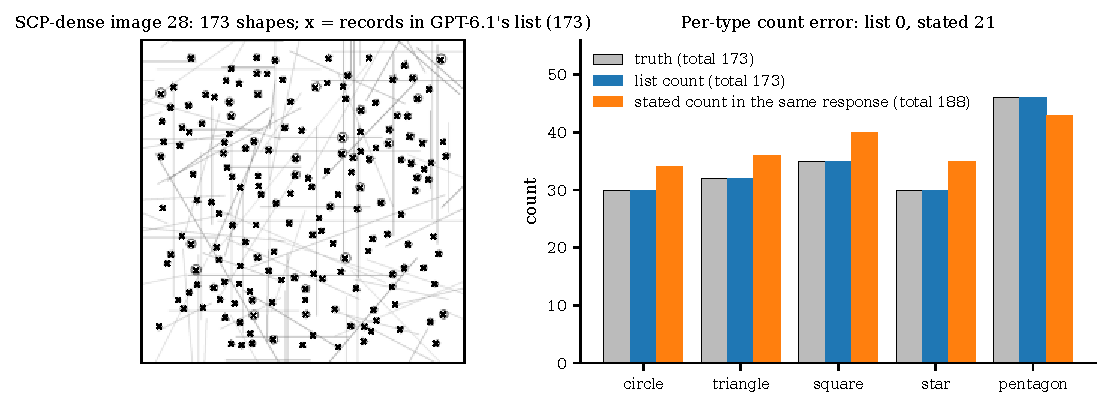
\includegraphics[width=\textwidth]{figures/fig_example.pdf}
\caption{One response, two answers. GPT-6.1 is asked to list every shape in a dense synthetic scene and then give counts by type ``for the shapes you listed''. The scene has 173 shapes. The list has 173 records, and each matches a different shape of the same class within 20 pixels, so the list count of every class is exact. The counts the model states in the same response sum to 188, and their per-type error is 21. Across 50 such scenes, list length misses the true total by 0.04 objects on average and the stated total misses by 7.78 (Table~\ref{tab:readout}). Image: SCP-dense 28; markers: centres in the model's list.}
\label{fig:example}
\end{figure*}

\paragraph{Same response, two answers.} Figure~\ref{fig:example} shows one response in full. When a list-first response has both a list and stated counts, the list length misses the true total by 0.04 objects on average for GPT-6.1 and 0.02 for Sonnet 5.5, while the stated totals miss by 7.78 and 10.48 (Table~\ref{tab:readout}, last row). Reading per-type counts from the list (the list count) instead of the stated counts in the same response cuts per-type count error by 75.6\% (GPT-6.1) and 77.7\% (Sonnet 5.5) under a count-first prompt, and by 84.2\% and 70.7\% under the list-first prompt. Generation is held fixed in these comparisons, so the gain is a readout effect: the model's list carries information that its own summary loses. Proposition~\ref{prop:readout} adds that the size of such a gap shows the two readouts are inconsistent but does not by itself say which one is right; here the labels say it is the list.

\paragraph{The gap grows with the length of a multi-type list.} Figure~\ref{fig:density} repeats the same-response comparison on four datasets. On PixMo (6 objects per image, one class) and FSC-147 (43.8 objects, one class), the stated total tracks the list for GPT-6.1 and Sonnet 5.5 and the difference is not significant. On SCP (47.6 objects, five classes) the list count is better by 44\% for GPT-6.1 and by 98.5\% for Sonnet 5.5, whose stated per-type counts are 65 times as far from the truth as its list. On SCP-dense (164.3 objects) both models gain 76\% to 78\%. The gap therefore appears when the stated count must summarize a long list across several classes, which is where practitioners most need counts.

\begin{figure*}[tp]
\centering
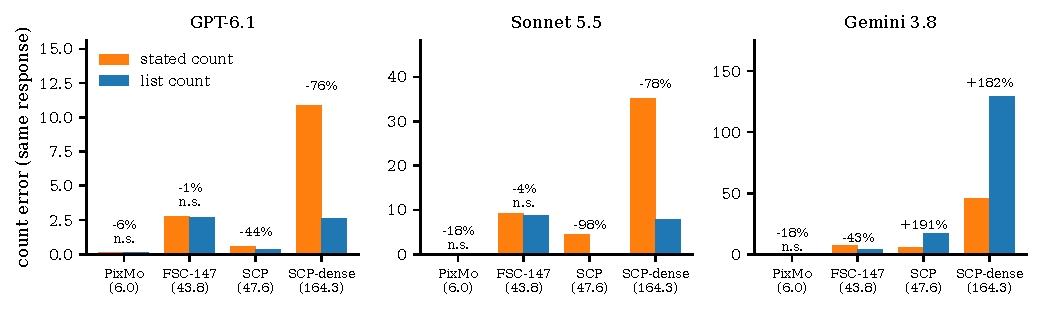
\includegraphics[width=\textwidth]{figures/fig_density.pdf}
\caption{Same-response readout across datasets, count-first prompts, lowest setting. Bars: count error of the stated count and of the list count (without the alias map) in the same response (per-type error on SCP and SCP-dense; total error on PixMo and FSC-147). Labels: relative change from stated count to list count; n.s.: paired 95\% interval includes 0. Numbers under dataset names: mean objects per image. Each panel has its own vertical scale. Gemini 3.8's lists degenerate on the synthetic scenes, so reading them is worse (Section~\ref{sec:res:degen}).}
\label{fig:density}
\end{figure*}

\paragraph{Aliases and protocol.} In list-first responses, Sonnet 5.5 wrote 258 ``diamond'' records across 50 images although the format listed the allowed names. The declared alias map, applied to the same list, takes its error from 5.42 to 0.42 ($-92.3\%$). The prompt alone does not do this: the map is part of the task, and the decoder applies it. Holding the mapped readout fixed, list-first lists are better than count-first lists by 39.4\% for GPT-6.1 and 92.3\% for Sonnet 5.5. The complete protocol, compared with the stated count of a count-first response, cuts error by 85.2\% $[-89.1,-80.3]$ for GPT-6.1 and 98.8\% $[-99.5,-98.1]$ for Sonnet 5.5. For Gemini 3.8 at its lowest setting the change is $+15.6\%$ $[-5.3,+39.4]$, not significant: the degeneracy check routes 40 of its 50 responses to the stated count. These are effects of the reporting and decoding protocol. The same-response and same-list comparisons isolate the readout and the alias map; the full protocol also changes how the list is generated, so it does not establish a change in perceptual ability either way.

\paragraph{Natural images with several classes.} The readout repair needs a gap to work with. We ran both prompts on 30 DOTA windows and 50 DocLayNet pages chosen to contain several classes and many objects (Table~\ref{tab:natural}; 574 calls). There the lists themselves miss objects: GPT-6.1 and Sonnet 5.5 list 68\% to 88\% of the true objects. The stated count also stays close to the list count of the same response, differing by 0.1 to 7.4 per image against per-type errors of 5 to 46. Switching readouts can change the error by at most this gap (Proposition~\ref{prop:readout}), so the change in the same response is small: none for GPT-6.1, and $-13.5\%$ and $-19.9\%$ for Sonnet 5.5. The full list-first protocol, here without the recovery step, changes count error by $+0.4\%$ and $-2.4\%$ for GPT-6.1 and by $-15.7\%$ and $-20.1\%$ for Sonnet 5.5, intervals reaching zero. Gemini 3.8 at its lowest setting again writes degenerate lists, the fallback to the stated count holds its change to $+18.0\%$ and $-7.9\%$, both not significant, and at its default setting, the shipped configuration, it lowers count error by 28.2\% on DOTA (interval reaching zero) and 25.8\% on DocLayNet. The two kinds of scene differ in where the error sits. On dense synthetic scenes the lists are nearly complete and the statement loses information, so the readout repairs most of the error; on these natural images most of the error is already in the list, so switching between the two readouts cannot remove it. The readout gap, which needs no labels, separates the two cases in one direction: a small gap shows that switching between the stated count and the list count can change the error by at most the gap, while a large gap shows only that the switch might matter. The gap says nothing about remedies that produce a new response.

\begin{table*}[tp]\centering\footnotesize\setlength{\tabcolsep}{3pt}
\caption{Readout on aerial and document images with several classes: 30 DOTA windows (71 objects and 3.3 classes per image on average) and 50 DocLayNet pages (25 elements, 5.0 classes); one call per image and arm, lowest setting unless stated, 16k cap. Per-type count error, lower is better; paired image bootstrap 95\% intervals. Difficult DOTA objects and objects less than half inside the window are not targets, so records on them are counted like any other record, for every readout alike. \emph{List recall}: share of true objects matched by a record centre inside a true box of the same class (list-first arm). \emph{Readout gap}: mean per-type difference between the stated count and the list count of the same count-first response, which bounds how much switching readouts can change the error. \emph{Same response}: stated count $\to$ list count of the count-first response. \emph{Full method}: readout of the list-first response (list count, or the stated count if the list is flagged) against the stated count of the count-first response; the Gemini 3.8 default row is the shipped configuration. \textbf{Bold}: the paired 95\% interval excludes 0 in the favourable direction; \underline{underlined}: it excludes 0 in the unfavourable direction.}\label{tab:natural}
\begin{tabular}{@{}llrrrrrr@{}}\toprule
& & & & \multicolumn{2}{c}{Same response} & \multicolumn{2}{c}{Full method} \\\cmidrule(lr){5-6}\cmidrule(l){7-8}
Images & Model & \begin{tabular}[b]{@{}c@{}}List\\recall (\%)\end{tabular} & \begin{tabular}[b]{@{}c@{}}Readout\\gap\end{tabular} & Error & Change, \% [95\% CI] & Error & Change, \% [95\% CI] \\\midrule
DOTA & GPT-6.1 & 88 & 2.2 & 40.5 $\to$ 40.8 & $+$0.7 [$-$5.0, 4.5] & 40.7 & $+$0.4 [$-$17.7, 16.4] \\
 & Sonnet 5.5 & 68 & 7.4 & 45.8 $\to$ 39.7 & {\bfseries\boldmath $-$13.5 [$-$34.7, $-$0.6]} & 38.6 & $-$15.7 [$-$38.2, 7.7] \\
 & Gemini 3.8 & 26 & 44.2 & 33.2 $\to$ 63.9 & \underline{$+$92.4 [54.2, 145.0]} & 39.2 & $+$18.0 [$-$13.4, 61.2] \\
 & Gemini 3.8, default & n/a & n/a & n/a & n/a & 23.9 & $-$28.2 [$-$48.6, 0.1] \\
\midrule
DocLayNet & GPT-6.1 & 87 & 0.1 & 4.9 $\to$ 4.9 & $+$0.4 [$-$1.6, 2.2] & 4.8 & $-$2.4 [$-$12.4, 4.5] \\
 & Sonnet 5.5 & 83 & 3.1 & 8.6 $\to$ 6.9 & {\bfseries\boldmath $-$19.9 [$-$32.5, $-$10.1]} & 6.8 & $-$20.1 [$-$36.7, 3.3] \\
 & Gemini 3.8 & 68 & 5.3 & 9.4 $\to$ 11.2 & \underline{$+$19.2 [1.6, 41.0]} & 8.6 & $-$7.9 [$-$24.7, 10.6] \\
 & Gemini 3.8, default & n/a & n/a & n/a & n/a & 7.0 & {\bfseries\boldmath $-$25.8 [$-$42.5, $-$8.8]} \\
\bottomrule\end{tabular}\end{table*}


\subsection{Repair the readout when the list degenerates}\label{sec:res:degen}

\begin{table*}[tp]\centering\footnotesize\setlength{\tabcolsep}{3pt}
\caption{Gemini 3.8 on SCP-dense under the list-first protocol (50 images, one call each). At a fixed 16k output cap, the default reasoning setting changes the count readout error by $-$53.6\% [$-$72.4, $-$29.5]; raising the cap to 32k changes it by a further $-$37.0\% [$-$62.4, 7.7] (not significant). Readout error: per-type count error of the Step-6 readout (stated count if the list is flagged, list count otherwise). List-count error: the same for the list count alone. Set error $E$ scores the delivered records, those whose class is valid after the alias map (equal class, 20 px); unknown-class records are excluded from the delivered set and counted in the next column; the column after it is a sensitivity that keeps them and scores them as unmatched. Flagged: share of lists with at least one degeneracy flag. JSON fail: share of responses that do not parse as the requested object (records are then recovered by the declared salvage step). Hit cap: share of responses that stopped at the output cap. Reasoning: share of calls with reasoning tokens. Output tokens: mean per call. Cost: all 50 calls, counting every attempted call. The setting comparison is cap-matched, not cost-matched: output tokens and cost rise with reasoning.}\label{tab:setting}
\begin{tabular}{@{}lrrrrrrrrrrr@{}}\toprule
\begin{tabular}[b]{@{}c@{}}Setting,\\cap\end{tabular} & \begin{tabular}[b]{@{}c@{}}Readout\\error\end{tabular} & \begin{tabular}[b]{@{}c@{}}List-count\\error\end{tabular} & \begin{tabular}[b]{@{}c@{}}Set\\error $E$\end{tabular} & \begin{tabular}[b]{@{}c@{}}Unknown\\records\end{tabular} & \begin{tabular}[b]{@{}c@{}}$E$, unknown\\kept\end{tabular} & \begin{tabular}[b]{@{}c@{}}Flagged\\(\%)\end{tabular} & \begin{tabular}[b]{@{}c@{}}JSON\\fail (\%)\end{tabular} & \begin{tabular}[b]{@{}c@{}}Hit\\cap (\%)\end{tabular} & \begin{tabular}[b]{@{}c@{}}Reasoning\\(\%)\end{tabular} & \begin{tabular}[b]{@{}c@{}}Output\\tokens\end{tabular} & \begin{tabular}[b]{@{}c@{}}Cost\\(\$)\end{tabular} \\\midrule
lowest, 16k & 52.80 & 96.78 & 103.46 & 184.76 & 288.22 & 90 & 72 & 4 & 0 & 4,796 & 0.95 \\
default, 16k & 24.52 & 25.90 & 34.58 & 4.90 & 39.48 & 12 & 70 & 8 & 100 & 8,831 & 1.71 \\
default, 32k & 15.44 & 20.14 & 28.26 & 8.84 & 37.10 & 6 & 78 & 0 & 98 & 9,487 & 1.83 \\
\bottomrule\end{tabular}\end{table*}


Gemini 3.8 at its lowest setting writes long lists in which most records lack a valid class and some coordinates repeat, so the list count is far worse than its stated count ($+182.5\%$ in the same response; Figure~\ref{fig:density}). The four-part degeneracy check of Section~\ref{sec:method} flags 45 of its 50 dense-scene lists. For 40 of them the readout falls back to the stated count; the other 5 have no stated count and keep the list count with a status flag. On the GPT-6.1 and Sonnet 5.5 list-first responses it flags none.

The degeneration is a property of the setting, not of the model. At the same 16k output cap, Gemini's default setting reduces flagged lists from 90\% to 12\% and the readout error from 52.80 to 24.52 ($-53.6\%$ $[-72.4,-29.5]$; Table~\ref{tab:setting}). Doubling the cap to 32k gives a point estimate of 15.44, a further change that is not significant. Even then, Gemini's dense-count error is about ten times GPT-6.1's, and none of its 50 counts is exact. Strict JSON parsing fails for 70\% to 78\% of Gemini responses at every setting, so the declared record salvage of Section~\ref{sec:setup:contract} is a necessary part of the decoder, and its share is reported.

On the list-first responses of the readout experiment, applying the same check to existing responses recovers 68\% (SCP) and 58\% (SCP-dense) of Gemini's error relative to reading its list, and 42\% relative to the stated count on FSC-147. For Sonnet 5.5, whose lists are not degenerate, the cost of the check reaches $+23\%$ on SCP and $+13\%$ on SCP-dense (not significant; intervals $[0,57]$ and $[0,26]$). On the open model Qwen3-VL, with thresholds unchanged, it lowers SCP-dense error by 7\% $[-13,-1]$ relative to the stated count. Gemini's missing class fields follow a pattern: a record is more likely to omit its type when the previous record has the same type, and a row-by-row scan that interleaves types cuts its count error by 60\%, while grouping by type makes it worse.

\subsection{Repair the set: delete below the threshold, keep geometry separate}\label{sec:res:set}

\begin{table*}[tp]\centering\small\setlength{\tabcolsep}{4pt}
\caption{Confirmation by a partner call, split into selection and geometry (Propositions~\ref{prop:identity} and \ref{prop:geometry}). Each source has 9 base/partner pairs (3 base models $\times$ same-model or one of two other models), 60 images, one call each; values are per-image reductions of $E$ (positive is better). Both identities hold exactly on every image of every pair. \emph{Sign from 5 labels}: $p_1$ is estimated on 5 labelled images and Proposition~\ref{thm:intersect} is used to predict whether deletion lowers $E$ on the other 55; the share of correct predictions over 200 draws per pair, averaged over the pairs (Section~\ref{sec:res:set}). Sign flips: pairs in which the fused total has the opposite sign of the deletion-only selection term. Full per-pair values are in Appendix~\ref{app:tables}.}\label{tab:intersect}
\resizebox{\textwidth}{!}{\begin{tabular}{@{}lcccccccc@{}}\toprule
Source & Pairs & Sign from 5 labels & Deletion helps & $p_1$ range & Selection range & Geometry $+$ / $-$ & Geometry range & Sign flips \\\midrule
DocLayNet & 9 & 74\% & 6 & 0.11 to 0.64 & $-$2.2 to 2.1 & 6 / 2 & $-$1.1 to 3.1 & 1 \\
DOTA & 9 & 98\% & 9 & 0.05 to 0.22 & 4.4 to 16.3 & 7 / 2 & $-$1.5 to 3.9 & 0 \\
FSC-147 & 9 & 81\% & 2 & 0.39 to 0.90 & $-$21.8 to 0.3 & 8 / 0 & 0.0 to 0.4 & 0 \\
SKU-110K & 9 & 96\% & 9 & 0.00 to 0.39 & 10.8 to 68.2 & 7 / 2 & $-$14.1 to 13.8 & 0 \\
GroundCUA & 9 & 86\% & 6 & 0.06 to 0.72 & $-$16.8 to 37.7 & 4 / 5 & $-$7.7 to 15.4 & 1 \\
ScreenParse & 9 & 63\% & 8 & 0.19 to 0.50 & 0.0 to 2.1 & 5 / 2 & $-$0.5 to 0.9 & 0 \\
\bottomrule\end{tabular}}\end{table*}


\paragraph{Deletion and geometry, measured separately.} Table~\ref{tab:intersect} splits the effect of confirming a base call with a partner call into the selection term of Proposition~\ref{prop:identity} and the geometry term of Proposition~\ref{prop:geometry}, for 54 base/partner pairs on six sources. Both identities hold exactly on every image, so the selection term of a pair has the sign of $1-2p_1$ by construction (Figure~\ref{fig:select}a). What the data add is where $p_1$ lies: 0.00 to 0.39 on SKU-110K and 0.05 to 0.22 on DOTA, where deletion removes 4 to 68 errors per image, against 0.39 to 0.90 on FSC-147. On FSC-147, where models under-report, $p_1$ is 0.39 to 0.90 and deletion hurts in 7 of 9 pairs, which is why counting families keep a single call. Coordinate averaging is positive in 37 pairs and negative in 13. In two pairs it reverses the sign of the deletion-only result: DocLayNet with GPT-6.1 confirmed by Sonnet 5.5 (selection $+0.80$, geometry $-1.10$ per image) and GroundCUA with Sonnet 5.5 confirmed by itself (selection $-0.87$, geometry $+1.20$). These are the two pairs in which an earlier check of the threshold on fused intersections failed; separating the terms accounts for both.

\paragraph{The threshold from a few labels.} The useful question is whether $p_1$ measured on a handful of labelled images predicts what deletion will do on other images. For each pair we drew 5 labelled images 200 times, estimated $p_1$ on them, and predicted from Proposition~\ref{thm:intersect} whether deleting unconfirmed records lowers set error on the other 55 images of the pair. The prediction is right in 83\% of draws (80\% with 3 labelled images, 87\% with 10), and the loss against the better decision on the other images is 0.33 errors per image (0.48 and 0.15). The shipped regime alone, which deletes on over-reporting families and keeps on FSC-147 without any label, is right in 85\% of draws with a loss of 0.43. The label rule of Step 7 combines the two: it starts from the regime and switches only if the labelled images favour the other decision by more than one standard error. It is right in 86\%, 87\% and 88\% of draws with 3, 5 and 10 labelled images, with losses of 0.22, 0.17 and 0.10 errors per image. In the 8 pairs whose $p_1$ lies within 0.1 of $1/2$, the gain from deleting is small and its sign is noisy: the plain threshold is right in 47\% of draws there, and the regime and the Step 7 rule, which lean towards deletion, in 34\% and 37\%. Table~\ref{tab:intersect} gives the share by source.

\begin{figure*}[tp]
\centering
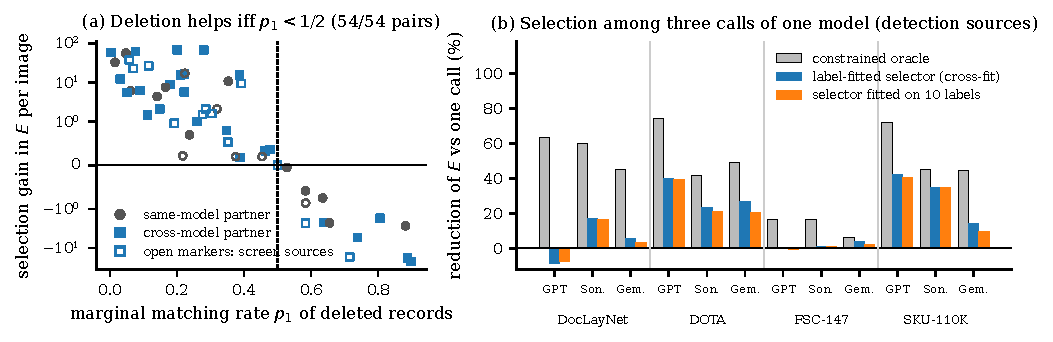
\includegraphics[width=\textwidth]{figures/fig_select.pdf}
\caption{(a) Selection gain of deleting unconfirmed records against their marginal matching rate $p_1$, for 54 base/partner pairs (symmetric log scale). With equal error costs the gain per image equals $\mathbb{E}[\Delta c](1-2p_1)$ exactly (Proposition~\ref{thm:intersect}), so this panel checks the implementation of an identity and shows how far each pair lies from the threshold; it is not an independent test. (b) Reduction of set error relative to one call when selecting among three calls of one model: constrained oracle, cross-fitted label-fitted selector, and the selector fitted on 10 labelled images (median of 40 draws).}
\label{fig:select}
\end{figure*}

\paragraph{Which partner helps.} Proposition~\ref{prop:partner} says a partner helps if it rejects more of the base call's false records than it loses of the true ones. Cross-model partners separate the two better than same-model partners in 32 of 36 base/partner comparisons on the E3 and screen-parsing sources. The four exceptions are GPT-6.1's two much weaker partners on FSC-147, and Gemini 3.8 confirming Sonnet 5.5 on FSC-147 and SKU-110K, where Gemini confirms few of Sonnet's true records. The misses are consistent with a component shared across models: of the objects that GPT-6.1, the highest-recall model, misses in all three of its calls, a single call of either other model recovers only 0.7\% to 9\% on SKU-110K, DOTA and FSC-147, and 18\% to 26\% on DocLayNet. New information flows mainly from higher-recall to lower-recall models.

\subsection{Repair the view; fixes that do not help}\label{sec:res:view}

\paragraph{Zoom and tiles.} Two-stage zoom clicks once on the whole screenshot, crops a third of each side around that point at native pixels, and clicks again in the crop; it is the re-grounding strategy that \citet{li2025screenspotpro} evaluate as ReGround. On ScreenSpot-Pro (200 items) it raises the click hit rate from 64.5\% to 87.5\% for Gemini 3.8 ($+23$ points $[16.5,29.5]$, a 65\% cut in click error) and from 78\% to 87\% for Sonnet 5.5 ($+9$ $[5,13.5]$, a 41\% cut; 45\% on the 196 items that every arm of Table~\ref{tab:common} answered); for GPT-6.1, 88.5\% to 90.0\% is not significant. Zooming only when two different models disagree, a cross-model version of the gated zoom in Table~\ref{tab:common}, is less accurate than zooming every item for Sonnet 5.5 (2.3 to 2.7 points) and Gemini 3.8 (9.6 to 12.3 points), no better for GPT-6.1, and more expensive. Our tiling arm on FSC-147 used $2\times2$ crops that overlap by 10\% of the side, each enlarged $2\times$ and sent in a separate call. It raises the tokens per object side for every object, but its overlap is smaller than one object for the larger objects (median exemplar side 17.5\% of the image side in the largest third), so it does not meet the companion paper's safe-decomposition condition that every target lie inside some view \citep{shi2026zoomin}. The results follow that condition. On the smallest third of images, Sonnet 5.5's count error falls by 70\% against whole-image lists; on the largest third, where many objects lie wholly inside no crop, GPT-6.1's rises by 78\%; over all images Sonnet's change ($-21\%$, $[-50,+27]$) is not significant. The small-object gain mixes more tokens per object with less content per call, and the large-object loss is consistent with objects that no crop contains rather than with object size as such. On screens, where tiles overlap by 6\%, objects cut by a tile boundary lose 0.16 to 0.42 in report probability in all 6 cells, and separate calls per tile beat one call with several tiles for GPT-6.1 ($-15\%$, $[-23,-5]$). For native-resolution click crops, downscaling costs Sonnet 5.5 9 points $[3,16]$, the loss for GPT-6.1 reaches 3 points ($[0,7]$, not significant), Gemini 3.8 shows no significant response to resizing, consistent with the fixed token grid measured for it in the companion paper, and enlarging these crops does not help.

\paragraph{Reports from a view planner.} In the cross-view experiment the pipeline receives, for each image, a whole-image report and four reports from four native-resolution crops (6\% overlap, one call per crop), on 30 GroundCUA screens and 30 SKU-110K images, scored at IoU $\ge0.5$ without class. Merging the four crop reports alone lowers set error relative to one whole-image call for GPT-6.1 on screens ($-19.4\%$ $[-27.5,-10.6]$) and for Sonnet 5.5 on SKU-110K ($-64.0\%$ $[-70.6,-56.6]$), raises it for Sonnet 5.5 on screens ($+44.9\%$) and for Gemini 3.8 on SKU-110K ($+24.7\%$), and is not significant in the other two cells. Confirming the whole-image report with the merged crops under the shipped rule, in which a crop confirms or rejects only the records it contains wholly, lowers set error in 4 of 6 cells: GPT-6.1 ($-22.8\%$) and Gemini 3.8 ($-20.3\%$) on screens, and GPT-6.1 ($-45.5\%$) and Sonnet 5.5 ($-36.6\%$) on SKU-110K. In these 4 cells it is also better than confirmation by a second whole-image call ($-11.8\%$ to $-22.6\%$), and better than the shipped three-call unanimity in 3 of them ($-8.0\%$ to $-20.2\%$; Gemini 3.8 on screens $-4.7\%$, not significant), at the price of five calls instead of three. In the other two cells it raises set error: Sonnet 5.5 on screens ($+12.9\%$) and Gemini 3.8 on SKU-110K ($+37.9\%$). The threshold of Proposition~\ref{thm:intersect} accounts for both groups. Among the whole-image records that the crops do not confirm, the share matched to a true object ($p_1$) is 0.03 to 0.24 in the four cells where confirmation helps, and 0.62 and 0.76 in the two where it hurts; this follows from an identity and is not an independent test. The plain rule, in which every record needs confirmation, differs from the shipped rule by at most 4 percentage points, because with a 6\% overlap few records lie wholly inside no crop.

\paragraph{Grids and coordinates.} On SCP, the systematic coordinate offset of current models is at most 0.3 pixels, with slope 1.000 and spread 0.9 to 1.5 pixels, against a matching tolerance of 30 pixels. A grid, ticks or cell labels therefore have no coordinate error to correct: in every arm, localization changes by at most 0.23 pixels, and at the lowest setting they do not change detection for GPT-6.1 and Sonnet 5.5. For Gemini 3.8 at its lowest setting, a grid lowers set error by 3.5 per image by reducing records that omit their class, and a row-by-row scan lowers it by 11.5; at its default setting the grid makes detection and localization slightly worse. ``No overlay'' is therefore the shipped default, chosen from these measurements; the theory does not forbid an overlay from helping a model whose list format it changes. Markers also make Sonnet 5.5 write ``diamond'' more often ($+0.3$ per image). An overlay on the sent image adds no Shannon information and can only change how the model uses its input \citep{shi2026zoomin}. We saw two such changes, fewer omitted class fields for Gemini 3.8 and more uses of the word ``diamond'' for Sonnet 5.5, and no coordinate correction, because on images within the vendors' budgets the offsets are about 1\% of the tolerance.

\paragraph{Wording, instructions and review.} ``Do not miss any'' wording, compared with a symmetric instruction not to miss or invent, has no measurable effect on SCP for any of the three models. Asking the model to localize each item relative to structures in the image has no significant effect, because current models have almost no location misses on these scenes. Same-view self-review, in which the model edits its own draft, confirms true and false records at nearly the same rate ($h_+\approx h_-$) and has no net gain on screen parsing; on FSC-147 it gave significant gains for 2 of 3 models, which we do not explain. Pairwise comparators that ask a model which of two reports is right judge whether something is an object rather than whether the box is precise, and are not used. Reasoning is not uniformly helpful: on 20 GroundCUA screens, GPT-6.1's default setting raises set error by 18.7 per screen $[5.8,34.3]$, through 16.3 additional false records and no fewer misses.

\subsection{Detect errors: they persist, so ask someone else}\label{sec:res:persist}

\paragraph{Persistence.} Object-level errors repeat across calls. Intraclass correlations of reporting across repeated calls are 0.60 to 0.98 for true objects and 0.23 to 0.93 for false reports. On the E3 sources, a binomial model with a common reporting probability is rejected in all 12 dataset and model cells, while a beta-binomial model fits. The share of misses that recur in every repeated call is 0.76 to 0.99 on the E3 sources and 0.73 to 0.94 on the screen sources. In clicks, 64\% to 83\% of a model's errors are repeated by a second call of the same model within the agreement tolerance.

\begin{figure*}[tp]
\centering
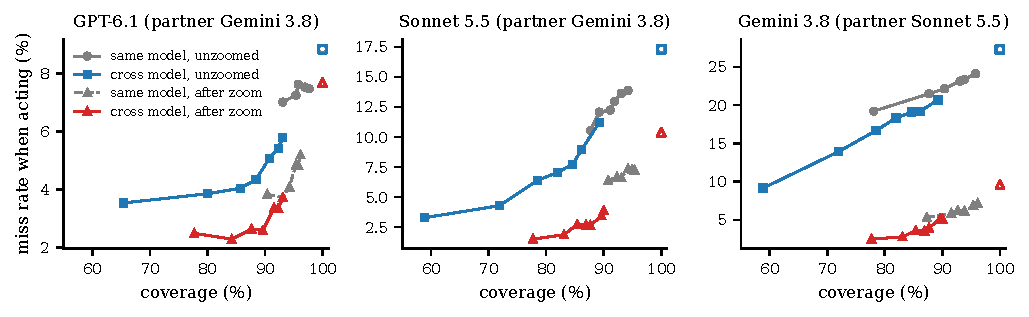
\includegraphics[width=\textwidth]{figures/fig_alarm.pdf}
\caption{Risk-coverage of click alarms (260 items). Each curve traces the alarm threshold $\delta\in\{0.5,1,1.5,2,3,5,8\}\%$ of the longer side; hollow markers at 100\% coverage are the error rates of acting on every item. The cross-model alarm (partner set by a fixed rule as the cheapest other model) reaches low-risk operating points that the same-model alarm does not; after two-stage zoom, the comparison of the two models' zoomed points gives the lowest risk.}
\label{fig:alarm}
\end{figure*}

\paragraph{A second model is a better alarm.} Persistence means that a second call of the same model rarely disagrees with the first where the first is wrong. A second model shares only part of the propensity. With the partner set by a fixed rule as the cheapest other model, the share of errors in which both calls agree on the same wrong point falls from 83\% to 39\% for GPT-6.1, from 64\% to 29\% for Sonnet 5.5, and from 73\% to 48\% for Gemini 3.8. At $\delta=1.5\%$, the same-model alarm catches 17\% of GPT-6.1's errors (4 of 23) and the cross-model alarm catches 61\% (14 of 23); for Sonnet 5.5 the shares are 36\% and 71\% (Table~\ref{tab:alarm}). The cross-model alarm defers more items, and Figure~\ref{fig:alarm} shows the trade-off: where the two curves overlap, its miss rate at matched coverage is lower by 0.4 to 2.7 points (point estimates on 260 items, without intervals), and for GPT-6.1 and Sonnet 5.5 it reaches operating points with a miss rate of 3\% to 4\%, below the lowest same-model values (7.0\% and 10.5\%). After two-stage zoom, which we compared only across models, comparing the two models' zoomed points still catches 68\% to 78\% of the remaining errors at $\delta=1.5\%$, with miss rates of 2.6\% to 3.6\% on the 85\% to 88\% of items acted on.

\begin{table*}[tp]\centering\footnotesize\setlength{\tabcolsep}{4pt}
\caption{Disagreement alarms for clicks (ScreenSpot-Pro and ScreenSpot-v2, 260 items; partner set by a fixed rule as the cheapest other model; point estimates). The alarm compares the acted-on point with a second point for the same item and fires when the two are farther apart than $\delta=1.5\%$ of the longer image side; in this risk-coverage analysis the item is then set aside instead of acted on (in Algorithm~\ref{alg:clicks} it triggers a comparison instead). Unzoomed alarms compare first clicks; after zoom, the acted-on point is the zoomed first click, and the second point is the same model's zoomed second click or the partner's zoomed first click. Miss rate, all items: miss rate when acting on every item. Acceptance coverage: share of items acted on. Miss rate when acting: share of acted-on items whose point is outside the target. Errors caught: share of the acted-on prediction's misses that the alarm sets aside. Other values of $\delta$ are in Figure~\ref{fig:alarm}, and miss rates at matched acceptance coverage in Table~\ref{tab:alarm_matched}.}\label{tab:alarm}
\begin{tabular}{@{}lllrrrr@{}}\toprule
Model & Partner & Alarm & \begin{tabular}[b]{@{}c@{}}Miss rate,\\all items (\%) $\downarrow$\end{tabular} & \begin{tabular}[b]{@{}c@{}}Acceptance\\coverage (\%) $\uparrow$\end{tabular} & \begin{tabular}[b]{@{}c@{}}Miss rate when\\acting (\%) $\downarrow$\end{tabular} & \begin{tabular}[b]{@{}c@{}}Errors\\caught (\%) $\uparrow$\end{tabular} \\\midrule
GPT-6.1 & Gemini 3.8 & same model, unzoomed & 8.9 & 95.8 & 7.6 & 17 \\
 &  & cross-model, unzoomed & 8.9 & 85.8 & 4.0 & 61 \\
 &  & same model, after zoom & 7.7 & 94.2 & 4.1 & 50 \\
 &  & cross-model, after zoom & 7.7 & 87.7 & 2.6 & 70 \\
\midrule
Sonnet 5.5 & Gemini 3.8 & same model, unzoomed & 17.3 & 91.1 & 12.2 & 36 \\
 &  & cross-model, unzoomed & 17.3 & 78.5 & 6.4 & 71 \\
 &  & same model, after zoom & 10.4 & 93.1 & 6.6 & 41 \\
 &  & cross-model, after zoom & 10.4 & 85.4 & 2.7 & 78 \\
\midrule
Gemini 3.8 & Sonnet 5.5 & same model, unzoomed & 27.3 & 90.4 & 22.1 & 27 \\
 &  & cross-model, unzoomed & 27.3 & 78.5 & 16.7 & 52 \\
 &  & same model, after zoom & 9.6 & 92.7 & 6.2 & 40 \\
 &  & cross-model, after zoom & 9.6 & 85.4 & 3.6 & 68 \\
\bottomrule\end{tabular}\end{table*}


\paragraph{Re-asking a failed call.} Because errors persist, re-asking also rarely repairs a failed call: in the detection experiments, resending the same request cleared 14.7\% of status flags that had already repeated, while changing the request cleared 58.8\% (Step 3 of Section~\ref{sec:method}).

\subsection{Judge: selection has room left, but labels do not close it}\label{sec:res:select}

\begin{table*}[tp]\centering\footnotesize\setlength{\tabcolsep}{2pt}
\caption{Selection among three calls of one model (detection sources, list interface, lowest setting, 60 images per cell; reduction of $E$ relative to the first call, in \%, higher is better). The constrained oracle optimizes over the same feasible family as the selectors (Proposition~\ref{prop:oracle}); the unrestricted value lets two members of one cluster match two targets and is not attainable. The two oracles differ on 25 of 720 images. Selectors are logistic or boosted-tree record gates on output features; they read no labels at inference but are fitted with labels: cross-fitted (5 folds by image, persisted), in-sample, or on 10 labelled images (median over 40 draws, each evaluated on the images it did not use). Gap: constrained oracle minus cross-fitted logistic, with a 95\% image-bootstrap interval for the fitted selector; it mixes information absent from the features with selector and estimation shortfall (Proposition~\ref{prop:order}).}\label{tab:select}
\begin{tabular}{@{}llrrrrrrr@{\hspace{8pt}}r@{}}\toprule
& & \multicolumn{2}{c}{Oracles} & \multicolumn{5}{c}{Selectors fitted with labels} & \\\cmidrule(lr){3-4}\cmidrule(lr){5-9}
Source & Model & Constrained & Unrestricted & \begin{tabular}[b]{@{}c@{}}Cross-fit\\logistic\end{tabular} & \begin{tabular}[b]{@{}c@{}}Cross-fit\\trees\end{tabular} & \begin{tabular}[b]{@{}c@{}}In-sample\\logistic\end{tabular} & \begin{tabular}[b]{@{}c@{}}In-sample\\trees\end{tabular} & \begin{tabular}[b]{@{}c@{}}10 labels\\logistic\end{tabular} & \begin{tabular}[b]{@{}c@{}}Gap\\{}[95\% CI]\end{tabular} \\\midrule
DocLayNet & GPT-6.1 & 63.2 & 63.2 & $-$8.4 & $-$7.4 & 1.6 & 42.8 & $-$7.7 & 71.6 [60.1, 87.4] \\
DocLayNet & Sonnet 5.5 & 59.8 & 59.8 & 17.3 & 14.8 & 22.6 & 50.1 & 16.6 & 42.5 [34.2, 54.0] \\
DocLayNet & Gemini 3.8 & 45.2 & 45.2 & 5.9 & 1.3 & 6.9 & 37.6 & 3.2 & 39.3 [30.1, 50.3] \\
DOTA & GPT-6.1 & 74.3 & 74.4 & 39.9 & 39.6 & 40.4 & 52.1 & 39.6 & 34.4 [25.1, 42.6] \\
DOTA & Sonnet 5.5 & 41.9 & 41.9 & 23.3 & 22.6 & 24.1 & 31.1 & 21.3 & 18.6 [13.7, 25.1] \\
DOTA & Gemini 3.8 & 49.3 & 49.3 & 26.8 & 24.6 & 27.5 & 36.0 & 20.5 & 22.5 [16.7, 30.1] \\
FSC-147 & GPT-6.1 & 16.7 & 19.0 & 0.2 & $-$0.7 & 1.6 & 5.0 & $-$0.7 & 16.5 [7.6, 31.7] \\
FSC-147 & Sonnet 5.5 & 16.6 & 17.3 & 1.1 & 1.0 & 1.2 & 5.5 & 0.8 & 15.5 [10.6, 21.4] \\
FSC-147 & Gemini 3.8 & 6.0 & 6.2 & 3.9 & 4.1 & 4.2 & 4.6 & 2.0 & 2.1 [0.8, 4.0] \\
SKU-110K & GPT-6.1 & 71.8 & 71.8 & 42.0 & 39.9 & 42.2 & 46.8 & 40.7 & 29.8 [27.2, 32.7] \\
SKU-110K & Sonnet 5.5 & 45.3 & 45.3 & 34.9 & 34.8 & 35.1 & 37.0 & 34.6 & 10.3 [8.4, 12.6] \\
SKU-110K & Gemini 3.8 & 44.6 & 44.6 & 13.9 & 14.3 & 14.3 & 22.7 & 9.8 & 30.6 [26.4, 35.6] \\
\midrule
\multicolumn{2}{@{}l}{Median of 12 cells} & 45.2 & 45.2 & 15.6 & 14.6 & 18.4 & 36.5 & 13.2 & 26.1 \\
\bottomrule\end{tabular}\end{table*}


\paragraph{Selection among a model's own outputs.} Choosing the best feasible set from a model's own three calls would remove 45.2\% of set error relative to one call (median over 12 cells; Table~\ref{tab:select}), and 72\% to 74\% for GPT-6.1 on SKU-110K and DOTA. The constrained oracle differs from the unrestricted value on 25 of 720 images and has the same median. Record gates on output features, fitted with labels and evaluated by cross-fitting, reach 15.6\% (logistic) and 14.6\% (boosted trees); fitted on 10 labelled images they reach 13.2\%. The more flexible selector does not help under cross-fitting, and its in-sample value (36.5\%) is overfit. The empirical gap, median 26.1 points, combines information absent from the output features with selector and estimation shortfall (Proposition~\ref{prop:order}); our results bound it but do not apportion it. It measures the distance between the tested selectors and the best set in a fixed library of three calls, so it does not bound what adding calls or changing the library could gain. Within the operations we compared, the larger gains came from changing the information, a different view, model or readout, rather than from selecting among a model's own outputs.

\subsection{Judge: defaults that transfer}\label{sec:res:transfer}

\begin{table*}[tp]\centering\small\setlength{\tabcolsep}{2.6pt}
\caption{Defaults evaluated by leave-one-source-out transfer: for each source, the construction is the one that is best on the other five sources (same model only, or any construction including cross-model ones), and it is evaluated on the evaluated source against a single call of the user's model. Entries are relative changes of the loss (for $E$, negative is better; for F1, positive is better). \textbf{Bold}: paired 95\% interval excludes 0 in the favourable direction; \underline{underlined}: significantly worse. $^{\star}$: the user's model is the strongest single model on that source and loss. Every significantly worse cross-model entry carries a $\star$. Costs, recall and the chosen construction per cell are in Appendix~\ref{app:tables}.}\label{tab:transfer}
\resizebox{\textwidth}{!}{\begin{tabular}{@{}lcccccccccccc@{}}\toprule
& \multicolumn{6}{c}{Same model only} & \multicolumn{6}{c}{Any construction (incl.\ cross-model)} \\\cmidrule(lr){2-7}\cmidrule(l){8-13}
& \multicolumn{3}{c}{$E$} & \multicolumn{3}{c}{F1} & \multicolumn{3}{c}{$E$} & \multicolumn{3}{c}{F1} \\\cmidrule(lr){2-4}\cmidrule(lr){5-7}\cmidrule(lr){8-10}\cmidrule(l){11-13}
Source & GPT & Son. & Gem. & GPT & Son. & Gem. & GPT & Son. & Gem. & GPT & Son. & Gem. \\\midrule
DocLayNet & $+$7\%$^{\star}$ & \textbf{$-$10\%} & $+$3\% & \underline{$-$3\%}$^{\star}$ & $-$1\% & \textbf{$+$19\%} & $+$4\%$^{\star}$ & \textbf{$-$36\%} & \textbf{$-$13\%} & $-$7\%$^{\star}$ & \textbf{$+$15\%} & \textbf{$+$75\%} \\
DOTA & \textbf{$-$22\%} & \textbf{$-$16\%}$^{\star}$ & \textbf{$-$25\%} & $-$1\%$^{\star}$ & $-$1\% & $+$2\% & \textbf{$-$30\%} & \textbf{$-$17\%}$^{\star}$ & \textbf{$-$22\%} & $-$6\%$^{\star}$ & $+$11\% & \textbf{$+$17\%} \\
FSC-147 & $+$3\%$^{\star}$ & \underline{$+$7\%} & \underline{$+$5\%} & $-$2\%$^{\star}$ & \underline{$-$6\%} & $+$1\% & \underline{$+$58\%}$^{\star}$ & $-$1\% & $-$1\% & \underline{$-$35\%}$^{\star}$ & $+$1\% & \textbf{$+$68\%} \\
SKU-110K & \textbf{$-$25\%} & \textbf{$-$32\%} & \textbf{$-$10\%}$^{\star}$ & \underline{$-$8\%}$^{\star}$ & $+$1\% & \textbf{$+$13\%} & \textbf{$-$30\%} & \textbf{$-$36\%} & \textbf{$-$8\%}$^{\star}$ & \underline{$-$22\%}$^{\star}$ & \textbf{$+$165\%} & \textbf{$+$21\%} \\
GroundCUA & $-$4\% & $-$1\%$^{\star}$ & \textbf{$-$21\%} & \underline{$-$4\%} & $+$2\%$^{\star}$ & $+$12\% & \textbf{$-$26\%} & \underline{$+$52\%}$^{\star}$ & \textbf{$-$42\%} & \textbf{$+$24\%} & \underline{$-$17\%}$^{\star}$ & \textbf{$+$61\%} \\
ScreenParse & \textbf{$-$3\%} & $-$2\%$^{\star}$ & $-$3\% & 0\% & 0\%$^{\star}$ & $+$2\% & \textbf{$-$14\%} & $+$4\%$^{\star}$ & \textbf{$-$12\%} & \textbf{$+$6\%} & $-$2\%$^{\star}$ & \textbf{$+$11\%} \\
\midrule
Better / worse / n.s. & \multicolumn{3}{c}{9 / 2 / 7} & \multicolumn{3}{c}{2 / 4 / 12} & \multicolumn{3}{c}{12 / 2 / 4} & \multicolumn{3}{c}{10 / 3 / 5} \\
\bottomrule\end{tabular}}\end{table*}


Table~\ref{tab:transfer} evaluates construction transfer on stored reports: for each source, the construction that does best on the other five sources is applied to the stored calls of the sixth, so it is never chosen on the source it is evaluated on. Table~\ref{tab:defaults} shows where the final defaults follow these transferred constructions and where they differ. For set error, the best same-model construction on the other five sources is three-call unanimity with fused coordinates on every evaluated source. It lowers set error significantly in 9 of the 15 over-reporting cells and raises it in none; on FSC-147, the under-reporting family, it is worse in 2 of 3 cells, consistent with Proposition~\ref{thm:intersect} and Corollary~\ref{cor:nonid}. For F1, the transferred same-model construction is better in 2 cells, worse in 4 and not significant in 12, so the default is a single call. Three calls cost three times one call. From logged token usage at list prices, unanimity costs \$0.029 to \$0.21 per image for GPT-6.1 across the five over-reporting sources, \$0.032 to \$0.13 for Sonnet 5.5 and \$0.011 to \$0.058 for Gemini 3.8.

When cross-model constructions are allowed, the transferred default improves set error in 12 of 18 cells and F1 in 10 of 18. It is better in 20 of the 24 cells in which the user's model is not the strongest single model for that source and loss, and not significantly different in the other 4. All 5 cells in which it is significantly worse are cells where the user's model is the strongest; for example, a three-model majority raises Sonnet 5.5's set error on GroundCUA by 52\% relative to one call, and a two-model intersection raises GPT-6.1's on FSC-147 by 58\%. Against the best same-model construction chosen with all labels (a reference, not a deployable rule), the best cross-model construction is significantly better only on DOTA ($-5.8\%$) and significantly worse on GroundCUA ($+26.0\%$). When the user does not know which model is strongest, three-model unanimity is significantly better than three-call unanimity of a randomly chosen model on 4 of 5 over-reporting sources ($-4\%$ to $-11\%$). Voting a strong model together with weaker ones is not a safe default: a three-model majority is 52\% worse than GPT-6.1's own three-call majority on FSC-147 and 59\% worse than Sonnet 5.5's on GroundCUA, three-model click voting is 3.5 points below GPT-6.1 alone, and the per-type median of three models' dense counts is 0.60 worse than Sonnet 5.5 alone. On aerial and shelf detection the same vote helps instead: it is 9.5\% better than Sonnet 5.5's three-call majority on DOTA and 4.7\% better than Gemini 3.8's on SKU-110K; on DocLayNet and ScreenParse it is not significantly different. Cross-model confirmation is therefore a menu option chosen with a few labels or a family-level ranking, while the cross-model alarm is a default whenever a second model is available.

